\begin{appendices}
	
\chapter{Πρότυπα αρχεία παραγωγής κώδικα}
\label{appendix:templates}

Παρακάτω παρουσιάζονται τα διαγράμματα που παράχθηκαν κατά τη διαδικασία του M2M μετασχηματισμού, στα πλαίσια του παραδείγματος στο \autoref{sec:example1}.

\begin{lstlisting}[style=CStyle, title={Κύριο πρότυπο που καλεί και όλα τα υπόλοιπα}]
	#include <time.h>
	#include "shell.h"
	#include "msg.h"
	#include "fmt.h"
	#include "xtimer.h"
	#include "string.h"
	
	/* Peripheral includes */
	
	#include "{{ name }}.h"
	#include "{{ name }}_params.h"
	
		
	/* MQTT-S includes */
	#include "net/emcute.h"
	#include "net/ipv6/addr.h"
	
	#ifndef EMCUTE_ID
	#define EMCUTE_ID ("gertrud")
	#endif
	#define EMCUTE_PORT ({{ port }})
	#define EMCUTE_ADDRESS ("{{ address }}")
	
	#define NUMOFSUBS (16U)
	#define TOPIC_MAXLEN (64U)
	
	msg_t queue[8];
	
	static emcute_sub_t subscriptions[NUMOFSUBS];
	static char topics[NUMOFSUBS][TOPIC_MAXLEN];
	
	
	char stack{{ id[loop.index0] }}[THREAD_STACKSIZE_DEFAULT];
	
	char stack_mqtt[THREAD_STACKSIZE_DEFAULT];
	
	
		
	
	
	/*
	* [ {{name}} {{peripheral_type[name]}} ] 
	* This function gets a sensor measurement with frequency {{ frequency[loop.index0] }} Hz 
	* and publishes it to topic '{{ topic[loop.index0] }}'.
	*/
	
	/*
	* [ {{name}} {{peripheral_type[name]}} ] 
	* This function implements the action that the actuator will do in the event of a 
	* published message in the topic that it listens to ({{topic[loop.index0]}}).
	*/
	
	
	
	
	int main(void)
	{
		printf("This application runs on %s\n", RIOT_BOARD);
		
		/* Initialize our subscription buffers */
		memset(subscriptions, 0, (NUMOFSUBS * sizeof(emcute_sub_t)));
		
		/* Start the emcute thread */
		thread_create(stack_mqtt, sizeof(stack_mqtt), 
						THREAD_PRIORITY_MAIN - 1, 
						0,
						emcute_thread, 
						NULL, "emcute");
		
		/* Try to connect to the gateway */
		if (con(EMCUTE_ADDRESS, EMCUTE_PORT))
			printf("Couldn't connect to broker. The measurements will just be printed instead.\n");
		
		
		/* Start the {{ name }} thread*/
		thread_create(stack{{ id[loop.index0] }}, sizeof(stack{{ id[loop.index0] }}),
						THREAD_PRIORITY_MAIN - 1,
						THREAD_CREATE_STACKTEST,
						
						send_{{ name }},
						
						receive_{{ name }},
						
						NULL, "{{ name }}");
		
			
		return 0;
}
\end{lstlisting}

\newpage

\begin{lstlisting}[style=CStyle, title={Πρότυπο παραγωγής κώδικα για επικοινωνία MQTT}]
	void *emcute_thread(void *arg)
	{
		(void)arg;
		emcute_run(EMCUTE_PORT, EMCUTE_ID);
		return NULL; // should never be reached
	}
	
	/*
	* Function to get qos level
	*/
	unsigned get_qos(int qos)
	{
		switch (qos)
		{
			case 1:
			return EMCUTE_QOS_1;
			case 2:
			return EMCUTE_QOS_2;
			default:
			return EMCUTE_QOS_0;
		}
	}
	
	/*
	* Function that connects to the MQTT-SN gateway   
	*                                                 
	* - param addr    MQTT-SN Gateway IP address      
	* - param port    MQTT-SN Gateway Port            
	*/
	int con(char *addr, int port)
	{
		sock_udp_ep_t gw = {.family = AF_INET6, .port = EMCUTE_PORT};
		gw.port = port;
		
		/* parse address */
		if (ipv6_addr_from_str((ipv6_addr_t *)&gw.addr.ipv6, addr) == NULL)
		{
			printf("error parsing IPv6 address\n");
			return 1;
		}
		
		if (emcute_con(&gw, true, NULL, NULL, 0, 0) != EMCUTE_OK)
		{
			printf("error: unable to connect to [%s]:%i\n", addr, port);
			return 1;
		}
		
		printf("Successfully connected to gateway at [%s]:%i\n", addr, port);
		return 0;
	}
	
	/*
	* Function that disconnects from the MQTT-SN gateway
	*/
	int discon(void)
	{
		int res = emcute_discon();
		
		if (res == EMCUTE_NOGW)
		{
			puts("error: not connected to any broker");
			return 1;
		}
		else if (res != EMCUTE_OK)
		{
			puts("error: unable to disconnect");
			return 1;
		}
		
		puts("Disconnect successful");
		return 0;
	}
	
	/*
	* Function that publishes a message to a topic 
	*                                             
	* - param topic   Topic in which to publish    
	* - param data    Message to be published      
	* - param qos     Quality of service           
	*/
	int pub(char *topic, char *data, int qos)
	{
		emcute_topic_t t;
		unsigned flags = EMCUTE_QOS_0;
		
		/* parse QoS level */
		flags |= get_qos(qos);
		
		/* Get topic id */
		t.name = topic;
		if (emcute_reg(&t) != EMCUTE_OK)
		{
			puts("error: unable to obtain topic ID");
			return 1;
		}
		
		/* Publish data */
		if (emcute_pub(&t, data, strlen(data), flags) != EMCUTE_OK)
		{
			printf("error: unable to publish data to topic '%s [%i]'\n",
			t.name, (int)t.id);
			return 1;
		}
		
		printf("published %s on topic %s\n", data, topic);
		
		return 0;
	}
	
	int sub(char *topic, int qos, void *func)
	{
		unsigned flags = EMCUTE_QOS_0;
		
		/* parse QoS level */
		flags |= get_qos(qos);
		
		/* find empty subscription slot */
		unsigned i = 0;
		for (; (i < NUMOFSUBS) && (subscriptions[i].topic.id != 0); i++) {}
		if (i == NUMOFSUBS) 
		{
			puts("error: no memory to store new subscriptions");
			return 1;
		}
		
		subscriptions[i].cb = func;
		strcpy(topics[i], topic);
		subscriptions[i].topic.name = topics[i];
		if (emcute_sub(&subscriptions[i], flags) != EMCUTE_OK) {
			printf("error: unable to subscribe to %s\n", topic);
			return 1;
		}
		
		printf("Now subscribed to %s\n", topic);
		return 0;
	}
\end{lstlisting}

\newpage

\begin{lstlisting}[style=CStyle, title={Πρότυπο παραγωγής κώδικα για αισθητήρα BME680}]
	void *send_srf04(void *arg)
	{
		(void) arg;
		
		/* Name of the topic */
		char topic[32];
		sprintf(topic, "{{topic[loop.index0]}}");
		
		/* Allocate memory for the message to be published */
		char *msg = malloc(128);
		
		/* Fix port parameter for digital sensor */
		srf04_params_t my_params;
		
		/* PINS */
		my_params.trigger = GPIO_PIN( 0, {{args[loop.index0]["trigger"]}} );
		my_params.echo = GPIO_PIN( 0, {{args[loop.index0]["echo"]}} );
		
		/* Initialize gpio and interrupt */
		srf04_t dev;
		if (srf04_init(&dev, &my_params) == SRF04_OK)
		printf("SRF04 sensor connected\n");
		else
		printf("Failed to connect to SRF04 sensor\n");
		
		/* Print sensor output with frequency {{ frequency[loop.index0] }} Hz */
		while (true)
		{
			/* Get a sensor measurement */
			int dist = srf04_get_distance(&dev);
			
			if (dist == SRF04_ERR_INVALID) 
			{
				printf("Error: No valid measurement is available\n");
			}
			else if (dist == SRF04_ERR_MEASURING) 
			{
				printf("Error: measurement is in progress\n");
			}
			else
			{
				/* Create a message to be published */
				sprintf(msg, "{id: {{ id[loop.index0] }}, SRF04 "
					"Output: [Distance]: %.2f cm}\n", 
					(float)dist / 10);
					
					printf("%s", msg);
					
					/* Publish to the topic */
					pub(topic, msg, 0);
			}
				
			/* Sleep for {{ 1/frequency[loop.index0] }} seconds */
			xtimer_msleep( 1000 / {{ frequency[loop.index0] }} );
		}
		
		return NULL;
	}
\end{lstlisting}

\newpage

\begin{lstlisting}[style=CStyle, title={Πρότυπο παραγωγής κώδικα για αισθητήρα BME680}]
	void *send_bme680(void *arg)
	{
		(void) arg;
		
		/* Name of the topic */
		char topic[32];
		sprintf(topic, "{{topic[loop.index0]}}");
		
		/* Allocate memory for the message to be published */
		char *msg = malloc(128);
		
		bme680_t dev[BME680_NUMOF];
		bme680_params_t myparams[BME680_NUMOF];
		memcpy(&myparams, &bme680_params, sizeof(bme680_params_t));
		
		for (unsigned i = 0; i < BME680_NUMOF; i++) 
		{
			BME680_SENSOR(&dev[i]).amb_temp = 25;
			
			myparams[i].intf.i2c.addr = 0x{{ args[loop.index0]["slave_address"] }};
			
			printf("Initialize BME680 sensor %u ... ", i);
			if (bme680_init(&dev[i], &myparams[i]) != BME680_OK)
			puts("failed");
			else
			puts("OK");
		}
		
		/* Print sensor output with frequency {{ frequency[loop.index0] }} Hz */
		while (true)
		{
			struct bme680_field_data data;
			
			for (unsigned i = 0; i < BME680_NUMOF; i++) 
			{
				/* trigger one measuerment */
				bme680_force_measurement(&dev[i]);
				/* get the duration for the measurement */
				int duration = bme680_get_duration(&dev[i]);
				/* wait for the duration */
				xtimer_msleep(duration);
				/* read the data */
				int res = bme680_get_data(&dev[i], &data);
				
				if (res == 0 && dev[i].sensor.new_fields) 
				{
					/* Create a message to be published */
					sprintf(msg, "{id: {{ id[loop.index0] }}, BME680 Output: ");
						#ifndef MODULE_BME680_FP
						sprintf(msg + strlen(msg), 
						"[Temp] = %02d.%02d C, "
						"[Pressure] = %" PRIu32 " Pa, "
						"[Humidity] = %02" PRIu32 ".%03" PRIu32 " %%",
						data.temperature / 100, data.temperature % 100,
						data.pressure, data.humidity / 1000, data.humidity % 1000);
						
						/* Avoid using measurements from an unstable heating setup */
						if (data.status & BME680_GASM_VALID_MSK) 
						sprintf(msg + strlen(msg),
						", [Gas] = %" PRIu32 " ohms", data.gas_resistance);
						#else
						sprintf(msg + strlen(msg), 
						"[Temp] = %.2f C, "
						"[Pressure] = %.2f Pa, "
						"[Humidity] %.3f %%",
						data.temperature, data.pressure, data.humidity);
						
						/* Avoid using measurements from an unstable heating setup */
						if (data.status & BME680_GASM_VALID_MSK) 
						sprintf(msg + strlen(msg),
						", [Gas] = %.0f ohms", data.gas_resistance);
						#endif
						sprintf(msg + strlen(msg), "}\n");
					
					printf("%s", msg);                
					
					/* Publish to the topic */
					pub(topic, msg, 0);
				}
				else if (res == 0)
				printf("[bme680]: no new data\n");
				else 
				printf("[bme680]: read data failed with reason %d\n", res);
			}
			
			/* Sleep for {{ 1/frequency[loop.index0] }} seconds */
			xtimer_msleep( 1000 / {{ frequency[loop.index0] }} );
		}
		
		return NULL;
	}
\end{lstlisting}

\newpage

\begin{lstlisting}[style=CStyle, title={Πρότυπο παραγωγής κώδικα για αισθητήρα MPL3115A2}]
	void *send_mpl3115a2(void *arg)
	{
		(void) arg;
		
		/* Name of the topic */
		char topic[32];
		sprintf(topic, "{{topic[loop.index0]}}");
		
		/* Allocate memory for the message to be published */
		char *msg = malloc(128);
		
		/* Initialize the sensor*/
		mpl3115a2_t dev;
		int init = mpl3115a2_init(&dev, &mpl3115a2_params[0]);
		if ( init != MPL3115A2_OK )
		puts("Error: Failed to initialize device!");
		
		/* Activate measurement*/
		if (mpl3115a2_set_active(&dev) == MPL3115A2_OK)
		printf("MPL3115A2 sensor connected\n");
		else 
		printf("Failed to activate measurement\n");
		
		/* Print sensor output with frequency {{ frequency[loop.index0] }} Hz */
		while (true)
		{
			uint32_t pressure;
			int16_t temp;
			uint8_t status;
			
			if ((mpl3115a2_read_pressure(&dev, &pressure, &status) |
			mpl3115a2_read_temp(&dev, &temp)) != MPL3115A2_OK)
			{
				puts("Error: Failed to read values!");
			}
			else
			{
				/* Create a message to be published */
				sprintf(msg, "{id: {{ id[loop.index0] }}, MPL3115A2 Output: [Pressure]: %u Pa, "
					"[Temperature]: %3d.%d C, [State]: %#02x}\n",
					(unsigned int)pressure, temp / 10, abs(temp % 10), status);
					
					printf("%s", msg);
					
					/* Publish to the topic */
					pub(topic, msg, 0);
			}
				
			/* Sleep for {{ 1/frequency[loop.index0] }} seconds */
			xtimer_msleep( 1000 / {{ frequency[loop.index0] }} );
		}
			
		return NULL;
	}
\end{lstlisting}

\begin{lstlisting}[style=CStyle, title={Πρότυπο παραγωγής κώδικα για ενεργοποιητή WS281x}]
	void ws281x_on_pub(const emcute_topic_t *topic, void *data, size_t len)
	{
		char *msg = (char *)data;
		
		printf("### got publication for topic '%s' [%i] ###\n",
		topic->name, (int)topic->id);
		for (size_t i = 0; i < len; i++) {
			printf("%c", msg[i]);
		}
		puts("");
		
		/* Array to store splitted RGB values (as strings) */
		char **rgb_str = malloc(3 * sizeof(char*));
		for (int i = 0; i < 3; i++)
		rgb_str[i] = malloc(2 * sizeof(char));
		
		/* Array to store splitted RGB values (as integers) */
		int *rgb = malloc(3 * sizeof(int));
		
		ws281x_t dev;
		ws281x_params_t my_params;
		memcpy(&my_params, ws281x_params, sizeof(ws281x_params_t));
		int init;
		
		/* Connected input pin */
		my_params.pin = GPIO_PIN( 0, 0 );
		
		/* Number of LEDs to light up */
		my_params.numof = 12U;
		
		uint8_t buf[my_params.numof * WS281X_BYTES_PER_DEVICE];
		my_params.buf = buf;
		
		if ( (init = ws281x_init(&dev, &my_params)) != 0 )
		printf("WS281X initialization failed with error code %d\n", init);
		else
		printf("WS281X actuator initialized\n");
		
		/* Split message to RGB */
		for (int i = 0; i < 3; i++)
		{
			memcpy( rgb_str[i], &msg[2*i], 2 );
			rgb[i] = (int)strtol(rgb_str[i], NULL, 16);
		}
		
		/* Store RGB values in a data structure */
		color_rgb_t colors = { .r = rgb[0], .g = rgb[1], .b = rgb[2] };
		
		for (uint16_t i = 0; i < dev.params.numof; i++) 
		ws281x_set(&dev, i, colors);
		
		ws281x_write(&dev);
	}
	
	
\end{lstlisting}

\begin{lstlisting}[style=CStyle, title={Πρότυπο παραγωγής κώδικα για την subscriber συνάρτηση ενός ενεργοποιητή}]
	void *receive_{{ peripheral_name[loop.index0] }}(void *arg)
	{
		(void) arg;
		
		/* Name of the topic */
		char topic[32];
		sprintf(topic, "{{topic[loop.index0]}}");
		
		sub(topic, 0, {{ peripheral_name[loop.index0] }}_on_pub);
		
		return NULL;
	}
\end{lstlisting}

\newpage

\begin{lstlisting}[style=MakefileStyle, title={Πρότυπο παραγωγής αρχείου Makefile}]
	# name of your application
	APPLICATION = {{ connection_conf }}
	
	# If no BOARD is found in the environment, use this default:
	BOARD ?= {{ board_name }}
	
	# This has to be the absolute path to the RIOT base directory:
	RIOTBASE ?= $(HOME)/RIOT
	
	# Include Peripheral and FMT module
	
	USEMODULE += {{module}}
	
		
	USEMODULE += fmt
	USEMODULE += xtimer
	
	# Comment this out to disable code in RIOT that does safety checking
	# which is not needed in a production environment but helps in the
	# development process:
	DEVELHELP ?= 1
	
	# Change this to 0 show compiler invocation lines by default:
	QUIET ?= 1
	
	# Include packages that pull up and auto-init the link layer.
	# NOTE: 6LoWPAN will be included if IEEE802.15.4 devices are present
	USEMODULE += gnrc_netdev_default
	USEMODULE += auto_init_gnrc_netif
	# Specify the mandatory networking modules for IPv6
	USEMODULE += gnrc_ipv6_default
	# Include MQTT-SN
	USEMODULE += emcute
	# Add also the shell, some shell commands
	USEMODULE += shell
	USEMODULE += shell_commands
	USEMODULE += ps
	# For testing we also include the ping6 command and some stats
	USEMODULE += gnrc_icmpv6_echo
	# Optimize network stack to for use with a single network interface
	USEMODULE += gnrc_netif_single
	
	# Connect board to wifi
	USEMODULE += esp_wifi
	CFLAGS += -DESP_WIFI_SSID=\"{{wifi_ssid}}\"
	CFLAGS += -DESP_WIFI_PASS=\"{{wifi_passwd}}\"
	
	# Give specific ID to this MQTT node
	CFLAGS += -DEMCUTE_ID=\"{{ connection_conf }}\"
	
	include $(RIOTBASE)/Makefile.include	
\end{lstlisting}

\newpage

\begin{lstlisting}[style=CStyle, title={Πρότυπο παραγωγής κώδικα για μη υποστηριζόμενο αισθητήρα}]
	void send_{{ peripheral_name[loop.index0] }}(void *arg)
	{
		(void) arg;
		
		/* Name of the topic */
		char topic[32];
		sprintf(topic, "{{topic[loop.index0]}}");
		
		/* Allocate memory for the message to be published */
		char *msg = malloc(128);
		
		/*
		* You need to fill the rest of this function. This function should first initialize
		* the sensor, get a measurement, and then publish it to the broker. 
		*/
		
		return NULL;
	}
\end{lstlisting}

\begin{lstlisting}[style=CStyle, title={Πρότυπο παραγωγής κώδικα για μη υποστηριζόμενο ενεργοποιητή}]
	void {{ peripheral_name[loop.index0] }}_on_pub(const emcute_topic_t *topic, void *data, size_t len)
	{
		char *msg = (char *)data;
		
		printf("### got publication for topic '%s' [%i] ###\n",
		topic->name, (int)topic->id);
		for (size_t i = 0; i < len; i++) {
			printf("%c", msg[i]);
		}
		puts("");
		
		/*
		* You need to fill the rest of this function. This function should store
		* the published message, initialize the actuator and then act accordingly. 
		*/ 
	}
	
	
\end{lstlisting}

\chapter{Διαγράμματα}
\label{appendix:diagrams}

Παρακάτω παρουσιάζονται τα διαγράμματα που παράχθηκαν κατά τη διαδικασία του M2M μετασχηματισμού, στα πλαίσια του παραδείγματος της ενότητας \autoref{sec:example1}.

\begin{figure}[!ht]
	\centering
	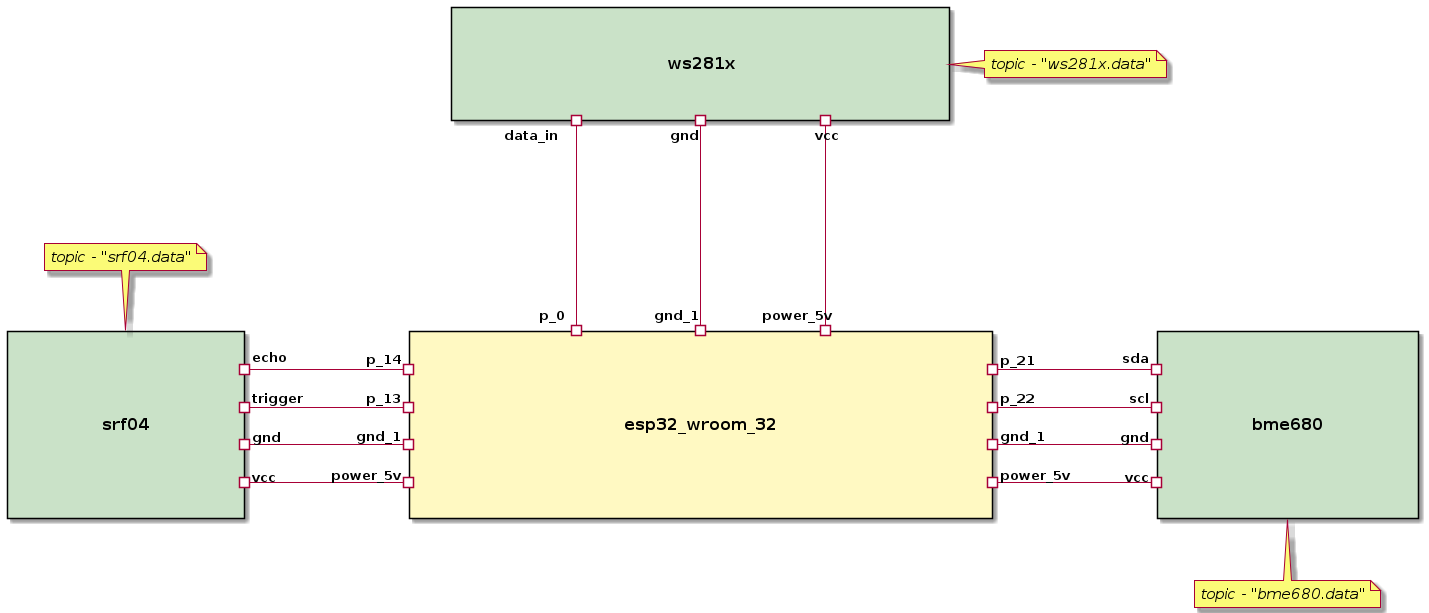
\includegraphics[width=1.0\textwidth]{./images/chapter6/example1a.png}
	\caption{Συνδεσμολογία μεταξύ των συσκευών}
	\label{fig:diagram_1}
\end{figure}

\begin{figure}[!ht]
	\centerline{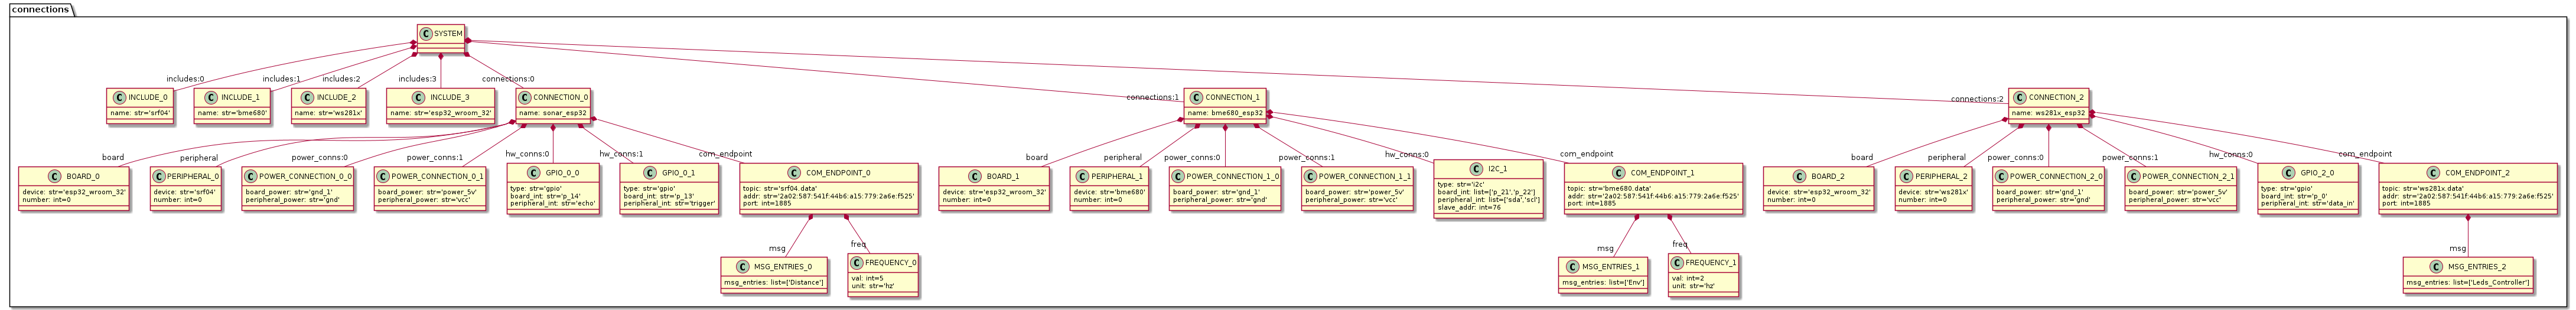
\includegraphics[width=0.9\paperwidth]{./images/chapter6/example1b.png}}
	\caption{Χαρακτηριστικά των συνδέσεων}
	\label{fig:diagram_2}
\end{figure}

\end{appendices}